\documentclass[10pt,a4paper]{article}
\usepackage[utf8]{inputenc}
\usepackage[italian]{babel}
\usepackage{amsmath}
\usepackage{amsthm}
\usepackage{amsfonts}
\usepackage{amssymb}
\usepackage{graphicx}
\usepackage[left=2cm,right=2cm,top=2cm,bottom=2cm]{geometry}
\usepackage{mathtools}
\author{Riccardo Pedrotti}

\title{Topology Groove - pt.1}

\theoremstyle{definition}
\newtheorem{defi}{Definizione}

\theoremstyle{plain}
\newtheorem{teo}{Teorema}
\newtheorem{cor}{Corollario}
\newtheorem{lem}{Lemma}
\newtheorem{prop}{Proposizione}

\theoremstyle{remark}
\newtheorem{rem}{Remark}
\theoremstyle{remark}
\newtheorem{ese}{Esempio}

\newcommand{\N}{\mathbb{N}}
\newcommand{\Q}{\mathbb{Q}}
\newcommand{\K}{\mathbb{K}}
\newcommand{\R}{\mathbb{R}}
\newcommand{\C}{\mathcal{C}}
\newcommand{\Hi}{\mathbb{H}}
\newcommand{\B}{\mathcal{B}}
\newcommand{\D}{\mathcal{D}}
\newcommand{\Ss}{\mathcal{S}}
\newcommand{\F}{\mathcal{F}}
\makeindex

\begin{document}
\maketitle
\vspace{2 cm}
\begin{center}
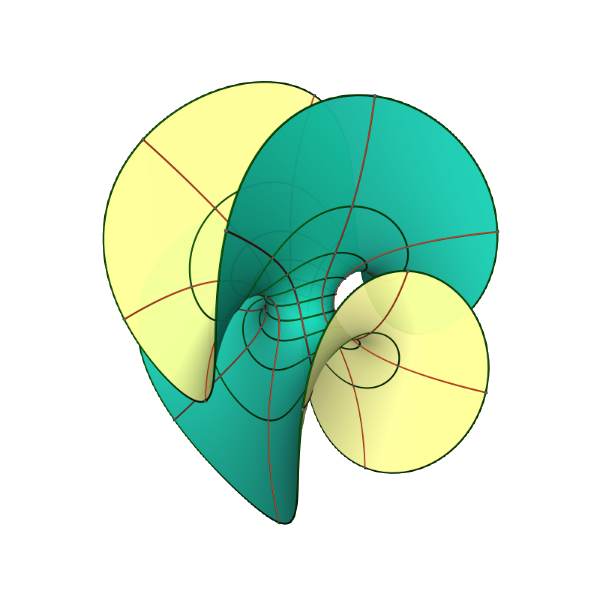
\includegraphics[scale=0.7]{enneper.png} 
\end{center}

\newpage


%Abbiamo solo due ore e quindi ho cercato di imbastire un percorso che lasci un pò di strumenti al matematico che deve affrontare, come me, questioni topologiche dalla mattina alla sera. In linea con lo spirito del Grappa di non essere un rimpiazzo delle lezioni di Geometria 2 ho imbastito un programmimo per il prossimo seminario che sia complementare a quello fatto a lezione e comunque spendibile anche per i non matematici:
%
%Ci concentreremo sul concetto di base per una topologia, per poi passare quasi naturalmente alle funzioni fra spazi topologici. Quindi continuità, l'essere aperta/chiusa e le varie condizioni equivalenti fra esse (alcune interessanti e che fa comodo ricordare). per concludere vorrei parlare di topologia indotta da una metrica, ma appena metto giù per iscritto i primi due blocchi avrò modo di decidere quanta profondità dare al terzo.
%
%Per via del tempo ristretto, scopo primario dell'intervento sarà appunto quello di rinfrescare alcuni strumenti classici nello studio della topologia generale, e di creare un pò di manualità ( che in fin dei conti è quello che serve avere per poi muoversi agevolmente in qualsiasi trattato sull'argomento). Sempre nello spirito del gruppo, si dimostrerà tutto quello che si enuncierà.
%
%Cose che NON riprenderò: cosa è una topologia, alcune costruzioni di topologie base (prodotto, indotta) le darò per assodate. Inoltre do epr buone, sebbene non vitali, chiusura, parte interna, hausdorff. Spero di aver elencato tutto.
%
%Come libro, seguirò il flow del Munkres, con qualche iniezione di Bourbaki in modo da rendere il più vivo possibile la narrazione: 

%pic here

%Il seguente schema è più per me che per tutti :P

\section{Base di una Topologia}

%Prima presentiamo una brevissima digressione sulla topologia, ispirato da un commento di un fisico che mi ha fatto martedì mattina\\



%\textit{Topology is the art of reasoning about imprecise measurements, in a sense I'll try to make precise.}\\ \textit{In a perfect world you could imagine rulers that measure lengths exactly. If you wanted to prove that an object had a length of $l$ you could grab your ruler marked $l$, hold it up next to the object, and demonstrate that they are the same length.} \\ \textit{In an imperfect world however you have rulers with tolerance. Associated to any ruler is a set $U$ with the property that if your length $l$ lies in $U$, the ruler can tell you it does. Call such a ruler $R_U$.}\\ \textit{Given two rulers $R_U$ and $R_V$ you can easily prove a length lies in $U \cup V$. You just hold both rulers up to the length and the length is in $U \cup V$ if one or the other ruler shows a positive match. You can think of $R_{U \cup V}$ as being a kind of virtual ruler.}\\ \textit{Similarly you can easily prove that a point lies in $U \cap V$ using two rulers.}\\ \textit{If you have an infinite family of rulers, $R_{U_i}$, then you can also prove that a length lies in $\bigcup_i U_i$. The length must lie in one of the $U_i$ and you simply exhibit the ruler $R_{U_i}$ matching for the appropriate $i$.}\\
%\textit{But you can't always do the same for $ \bigcap_i U_i$. To do so might require an infinitely long proof showing that all of the $R_{U_i}$ match your length.}\\ \textbf{A topology is a (generalised) set of rulers that fits this description}.\\ \textit{Your notion of ''measurement"" in whatever problem you have might not match the notion that the above description tries to capture. But to the extent that it does, topology will work as a way to reason about your problem.} \footnote{Tratto da http://mathoverflow.net/questions/19152/why-is-a-topology-made-up-of-open-sets}

%Partiamo quindi con alcuni concetti di basilare importanza:


\begin{defi}[Sistema Fondamentale di Intorni] Sia $X$ uno spazio topologico, un sistema fondamentale di intorni di un punto $x$ (risp. di un sottoinsieme $A$ di $X$) è una collezione $\mathcal{C}$ di intorni di $x$ (rispettivamente di $A$) tale per cui per ogni intorno $V$ di $x$ (risp. $A$) esiste un intorno $W \in \mathcal{C}$ tale che $W \subset V$.
\end{defi}


%\vspace{20 mm}

%Nei casi più semplici, riusciamo a descrivere una topologia fornendo esplicitamente ogni insieme aperto, nella realtà non sempre è possibile fare ciò e per questo dobbiamo trovare un modo formale di eliminare informazioni ridondanti, in un senso che spero sarà chiaro a fine percorso. Il concetto di base è ciò che ci permetterà di risparmiare qualcosa:

\begin{defi}[Base per una Topologia]  Sia $X$ un insieme. Una base per una topologia su $X$ è una collezione $\B$ di sottoinsiemi di $X$, chiamati elementi della base, tale che 
\begin{enumerate}
\item Per ogni $x \in X$, esiste almeno un elemento di $\B$ che contiene $x$
\item Se $x$ appartiame a due elementi della base $B_1, \ B_2$, allora esiste un elemento della base $B_3$ che contiene $x$ tale che $B_3 \subset B_1 \cap B_2$ 
\end{enumerate}

Se $\B$ soddisfa queste due condizioni, allora possiamo definire una topologia $\tau$ generata da $\B$ in questo modo: un sottoinsieme $U$ di $X$ è aperto in $X$ (cioè è un elemento di $\tau$) se per ogni $x \in U$, esiste un elemento $B$ della base $\B$ tale che $x \in B$ e $B \subset U$. Notiamo che ogni elemento della base è automaticamente aperto. 
\end{defi}

%\vspace{20 mm}

Ma è una topologia quella che abbiamo appena costruito?

\begin{enumerate}
\item $\emptyset \in \tau$. Infatti l'insieme vuoto verifica banalmente le richieste. (Per chi non fosse convinto, riuscite a trovare un elemento in $\emptyset$ che non sia contenuto in un elemento della base?)
\item $X \in \tau$ anche questo è banale, in quanto la base $\B$ ricopre $X$
\item Consideriamo l'unione arbitraria di elementi di $\tau$ $U= \bigcup_{\alpha}U_{\alpha}$. Mostriamo che siamo ancora in $\tau$. Sia $x \in U$, quindi esiste un indice $\alpha$ tale che $x \in U_{\alpha}$. Poiché $U_{\alpha} \in \tau$, cioè è aperto, esiste $B \in \B$ tale che $x \in B \subset U_{\alpha} \subset U$. Quindi $U$ è aperto per definizione.
\item Prendiamo ora due aperti $U_1, \ U_2$ e mostriamo che la loro intersezione è ancora aperta. Sia $x \in U_1 \cap U_2$. Per ipotesi esistono  due elementi della base che contengono il punto $x$, e più precisamente $B_1 \subset U_1, \ B_2 \subset U_2$. La seconda proprietà di una base per una topologia ci permette di scegliere un elemento della base $B_3$ che contiene $x$ e tale che $B_3 \subset B_1 \cap B_2$. $B_3$ è l'intorno di $x$ cercato che rende $U_1 \cap U_2$ un aperto.  Per induzione si verifica per ogni intersezione finita. 



\begin{center}
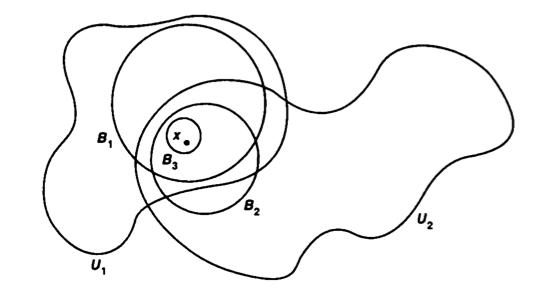
\includegraphics[scale=0.5]{intbase.png} 
\end{center}

\end{enumerate}


%\vspace{20 mm}

Un altro modo  per descrivere la topologia generata da una base $\B$ ci è data dal prossimo lemma

\begin{lem} Sia $X$ un insieme, sia $\B$ una base per una topologia $\tau$ su $X$. Allora $\tau$ è uguale alla collezione delle unioni arbitrarie di elementi di $\B$.
\end{lem}
\begin{proof}
Data una collezione di elementi di $\B$, loro sono ovviamente elementi di $\tau$. Poichè $\tau$ è una topologia, la loro unione è ancora in $\tau$. Al contrario, dato $U \in \tau$ , scegliamo per ogni $x \in U$ un elemento $B_x \in \B$ tale che $x \in B_x \subset U$. Allora $U = \bigcup_{x \in U} B_x$, quindi $U$ è uguale ad un'unione di elementi di $\B$.
\end{proof}

%\vspace{20 mm}
%Il lemma afferma che ogni aperto di una topologia è esprimibile come unione di elementi di una sua base. Ovviamente tale scrittura non è unica.
%
%Data una base, siamo in grado di generare una topologia a partire da essa. Certe volte siamo interessati a fare il processo contrario, cioè data una topologia ricavarne una base. 

\begin{lem}\label{baselem13.2} Sia $X$ uno spazio topologico. Supponiamo che $\C$ sia una collezione di aperti di $X$ tali che per ogni aperto $U$ di $X$ e per ogni $x$ in $U$, c'e un elemento $C$ di $\C$ tale che $x \in C \subset U$. Allora $\C$ è una base per la topologia di $X$. 
\end{lem}

\begin{proof}
Dobbiamo mostrare che $\C$ è una base. La prima condizione è facile: $X$ è aperto, e quindi per ogni suo $x \in X$ esiste un elemento $C$ di $\C$ che tale che $x \in C \subset X$. La seconda proprietà è facilmente verificata. $C_1 \cap C_2$ è ancora aperto e quindi per ipotesi esiste un elemento $C_3 \subset C_1 \cap C_2$

Sia ora $\tau$ la collezione degli aperti di $X$; vogliamo mostrare che la topologia $\tau'$ generata da $\C$ è uguale alla topologia $\tau$. Prima di tutto notiamo che se $U$ appartiene a $\tau$ e se $x \in U$, allora per ipotesi esiste $C \in \C$ tale che $x \in C \subset U$. Segue che $U$ appartiene a $\tau'$, per definizione. D'altro canto, se $W$ appartiene a $\tau'$ è unione di elementi della base che sono aperti in $\tau$, e quindi è aperto in $\tau$.
\end{proof}


%\vspace{20 mm}
%\begin{rem} esiste sempre una base topologica? Banalmente la risposta è si, in quanto la topologia stessa è una base per sè stessa. Bella forza direbbe qualcuno. Dal punto di vista teorico l'osservazione è molto importante: ci garantisce che concentrarci solo su di esse non è eccessivamente riduttivo. 
%\end{rem}

%Sempre sulla linea del presentare nozioni \textit{for the working mathematicians}, abbiamo la seguente


\begin{defi}[Prebase] Una prebase $\D$ per una topologia su $X$ è una collezione di sottoinsiemi di $X$ la cui unione copre tutto $X$. La topologia generata dalla prebase $\D$ è definita come la collezione di tutte le unioni delle intersezioni di elementi di $\D$.
\end{defi}
%\vspace{20 mm}
Dobbiamo ovviamente controllare che tale topologia generata (che chiameremo $\tau$) sia effettivamente una topologia. A tal riguardo ci basta controllare che la collezione $\B$ di tutte le intersezioni finite di elementi di $\D$ sia una base, dato che in quel caso abbiamo già verificato che genera una topologia. Dato $x \in X$ , esso appartiene ad un elemento di $\D$ e quindi ad un elemento di $\B$; questo è la prima condizione per una base. Per controllare anche la seconda definizione, sia \[ B_1=S_1 \cap \dots \cap S_m \ \ \ \text{ e } \ \ \ B_2=S_1' \cap \dots \cap S_n' \] due elementi di $\B$. La loro intersezione \[B_1 \cap B_2 = \left( S_1 \cap \dots \cap S_m \right) \cap \left( S_1' \cap \dots \cap S_n' \right) \] è ancora un intersezione finita di elementi di $\D$, e quindi appartiene a $\B$.

%\begin{rem} Differenze fra base e prebase: ho trovato su math.stackexchange.com questa domanda, sotto alla quale vi era la seguente interessante osservazione: \\ \textit{ Bases and subbases "generate" a topology in different ways. Every open set is a union of basis elements. Every open set is a union of finite intersections of subbasis elements. \\ For this reason, we can take a smaller set as our subbasis, and that sometimes makes proving things about the topology easier. We get to use a smaller set for our proof, but we pay for it; with a subbasis we need to worry about finite intersections, whereas we did not have to worry about that in the case of a basis.}\footnote{http://math.stackexchange.com/a/449577/74013}
%\end{rem}

Definiamo brevemente, non nella massima generalità, la topologia prodotto con cui viene equipaggiato solitamente il prodotto cartesiano di due spazi topologici:
\begin{defi}[Topologia Prodotto] Siano $X$ e $Y$ spazi topologici. La topologia prodotto su $X \times Y$ è la topologia avente come base la collezione $\B$ di tutti gli insiemi della forma $U \times V$, dove $U$ è un aperto in $X$ e $V$ è un aperto in $Y$.
\end{defi}


I controlli che siano una base per la topologia sono abbastanza ovvi e non li riportiamo. \\
%Alla luce del discorso sulle basi fatto fino ad ora, ci chiediamo se possiamo essere un po' più parsimoniosi introducendo una base 
\begin{teo} Se $\B$ è una base per la topologia di $X$ e $C$ è una base per la topologia di $Y$, allora la collezione \[ \D = \lbrace B \times C \mid  B \in \B \text{ e } C \in \C \rbrace \] è una base per la topologia di $X \times Y$.
\end{teo}
\begin{proof}
Vogliamo applicare il lemma \ref{baselem13.2}. Sia $W$ aperto di $X \times Y$ e sia $(x,y) \in W$, per definizione della topologia prodotto, esiste un aperto della forma $U \times V$, con $U,V$ aperti nelle rispettive topologie, tale che $(x,y) \in U \times V \subset W$. Poiché $\B$ e $\C$ sono basi per $X$ e $Y$ rispettivamente, possiamo scegliere un elemento $B \in \B$ tale che $x \in B \subset U$, e un elemento $C \in \C$ tale che $y \in C \subset V$. Ma allora $(x,y) \in B \times C \subset W$. Quindi per il lemma \ref{baselem13.2} la collezione $\D$ è una base. 
\end{proof}

%\vspace{20 mm}
Cerchiamo una prebase di questo spazio:\\
Siano $\pi_1 : X \times Y \to X$ e $\pi_2X \times Y \to Y$ le due mappe proiezione al primo e secondo fattore rispettivamente. Senza introdurre per ora il concetto di continuità notiamo che la controimmagine di un aperto via le due proiezioni è un aperto nella topologia prodotto $X \times Y$. Abbiamo quindi il seguente 

%\vspace{30 mm}
%\vspace{10 mm}
\begin{teo} La collezione \[ \Ss = \lbrace \pi_1^{-1}(U) \mid U \text{ aperto in } X \rbrace \cup \lbrace \pi_2^{-1}(V)\mid V \text{ aperto in } Y \rbrace \] è una prebase per la topologia prodotto $X \times Y$.
\end{teo}

\begin{proof}


Sia $\tau$ la topologia su $X \times Y$ e sia $\tau'$ la topologia generata da $\S$. Poichè ogni elemento di $\Ss$ appartiene alla topologia $\tau$, così anche le unioni arbitrarie delle loro intersezioni ci appartengono, e quindi $\tau' \subset \tau$. D'altra parte, ogni elemento della base $U \times V$ per la topologia $\tau$ è una intersezione finita di elementi di $\Ss$, in quanto \[ U \times V = \pi_1^{-1}(U) \cap \pi_2^{-1}(V) \] e quindi, $U \times V$ appartiene a $\tau'$, e quindi $\tau \subset \tau'$ che conclude la dimostrazione.
\end{proof}

\begin{center}
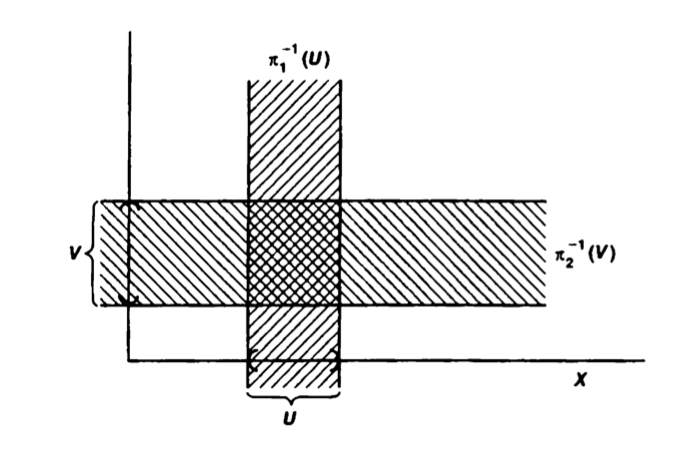
\includegraphics[scale=0.5]{prebaseprod.png} 
\end{center}


%\vspace{20 mm}

%Per completezza, e perchè lo useremo, definiamo il concetto di chiusura e di parte interna di un sottoinsieme di uno spazio topologico. Naturalmente, \textit{i chiusi sono definiti come i complementari degli aperti} e l'operazione di complementazione verrà indicata mettendo come apice una $c$.

\begin{defi}[Chiusura] la chiusura di $A$, denotata con $\text{cl}A$ o $\overline{A}$ è l'intersezione di tutti i chiusi che contengono $A$.
\end{defi}
%\vspace{20 mm}

\begin{defi}[Parte Interna] la parte interna di $A$, denotata con $\text{int}A$ è l'unione di tutti gli aperti contenuti in $A$.
\end{defi}

%\vspace{20 mm}
\begin{teo} Sia $A$ un sottoinsieme dello spazio topologico $X$.
\begin{enumerate}
\item $x \in \overline{A}$ se e solo se ogni aperto $U$ che contiene $x$ interseca $A$.
\item Possiamo restringere la condizione nel punto $(1)$ solo agli elementi di una base $\B$ di $X$
\end{enumerate}
\end{teo}
\begin{proof}
\begin{enumerate}
\item Dimostriamo l'equivalenza delle negazioni. Se $x$ non sta nella chiusura di $A$, allora l'insieme $U= \overline{A}^c$ è un aperto che contiene $x$ e che non interseca $A$, come desiderato. Al contrario, se esiste un aperto $U$ che contiene $x$ e che non interseca $A$, allora $U^c$ è chiuso e contiene $A$. Per definizione di chiusura di $A$, l'insieme $U^c$ deve contenere $\overline{A}$ e quindi $x$ non può stare in $\overline{A}$
\item Segue facilmente da quanto già provato. Se ogni aperto che contiene $x$  interseca $A$, allora anche ogni elemento della base, in quanto aperto. Al contrario, Se ogni elemento della base contenente $x$ interseca $A$, allora lo fa anche ogni aperto che contiene $x$, in quanto $U$ contiene un elemento della base che contiene $x$.
\end{enumerate}
\end{proof}

%\vspace{20 mm}
%Quasi dimenticavo, poichè gli insiemi chiusi sono tanto importanti quanto quegli aperti, si può definire un concetto di base duale, e risportare tutte le nozioni appena viste in termini di questa nuova base, avendo l'accortezza di sostituire $\bigcup$ con $\bigcap$.
\begin{defi}[Base per Insiemi Chiusi] Dato uno spazio topologico $X$, una base per gli insiemi chiusi di $X$ è una famiglia di insiemi chiusi $\F$ tale che ogni insieme chiuso $A$ di $X$ è esprimibile come intersezione arbitraria di elementi di $\F$.
\end{defi}

%\vspace{20 mm}
\begin{rem} la definizione di base per chiusi implica che $X$ ci deve appartenere. Quindi sarebbe superfluo richiedere che gli elementi di tale base ricoprano tutto $X$.
\end{rem}

%\vspace{20 mm}
%Alla domanda, mi esibisca una base di chiusi per $\R^n$ con la topologia indotta dalla metrica euclidea, si potrebbe rimanere un po' spiazzati. Ecco che il prossimo risultato può venire in aiuto
\begin{prop} $\F$ è una base per i chiusi in $X$ se e solo se la famiglia dei complementi è una base (nel senso standard) per $X$.
\end{prop}
\begin{proof}
immediata applicazione delle leggi di De Morgan. ($(A \cap B)^c= A^c \cup B^c$ e $(A \cup B)^c= A^c \cap B^c$)
\end{proof}

%\vspace{20 mm}
Analogamente abbiamo un'altra caratterizzazione per le basi dei chiusi

\begin{prop} Sia $\F$ una base per gli insiemi chiusi di $X$. Allora,
\begin{enumerate}
\item $\bigcap F = \emptyset$
\item per ogni $F_1$ e $F_2$ in $\F$, l'unione $F_1 \cup F_2$ è l'intersezione di qualche sottofamiglia di $\F$
\end{enumerate}
Inoltre ogni collezione di insiemi $x$ che soddisfa queste proprietà forma una base per i chiusi di una topologia di $X$. Gli insiemi chiusi in questa topologia saranno precisamente le intersezioni di sottofamiglie di $\F$.
\end{prop}
\begin{proof}
Se $\F$ è una base, allora la condizione $(1)$ è vera: $\empty$ è chiuso e quindi deve esistere una sottofamiglia disgiunta di elementi di questa base. Il punto $(2)$ è un'ovvia rilettura duale della proprietà di base topologica. Al contrario, se $\F$ soddisfa $(1)$ e $(2)$, possiamo costruire una topologia su $X$ i cui chiusi siano le intersezioni arbitrarie di tali elementi. Essa per $(1)$ e $(2)$ verificherà gli assiomi di topologia data in termini di chiusi. 
%
\end{proof}

%\vspace{20 mm}
%\begin{rem} Ci manca da verificare che se $X$ è uno spazio topologico (con $\tau$ la sua topologia) e $\F$ una base per i chiusi della topologia su $X$, allora la topologia generata da $\F$ (che chiameremo $\tau'$) e quella già presente coincidono. Ma come nel caso della base aperta, anche questo è ovvio: $X$ e $\emptyset$ sono chiusi per entrambe le topologie. Sia $C$ un chiuso per $\tau$, per definizione di base per i chiusi, $C = \bigcap F_{\alpha}$ e quindi $C $è chiuso anche per $\tau'$. Analogamente se $C$ è chiuso per $\tau'$ è anche chiuso per $\tau$. 
%\end{rem}
%\vspace{30 mm}
%\vspace{20 mm}
%Cosa servono le basi per i chiusi? beh ad esempio la topologia di Zarisky su uno spazio affine $n-$dimensionale è definita ponendo gli insiemi degli zeri delle funzioni polinomiali come base per i chiusi.


\section{Continuità di una funzione}
%La nozione di continuità è una di quelle nozioni essenziali che chiunque debba fare della matematica deve saper masticare. Nei corsi di analisi la tipica definizione di continuità è quella caratterizzata dagli $\varepsilon - \delta$, che in soldoni può essere tradotta in questo modo: \textit{Se vogliamo ottenere valori di $f(x)$ contenuti in un intorno di $f(c)$, ci basta semplicemente scegliere delle $x$ sufficientemente vicine a $c$.}
%\textit{Se questo vale per ogni intorno di $f(c)$, allora la funzione si dirà continua in $c$.}
%
%Poichè la nozione di distanza, usata per formulare tale definizione, può rivelarsi un ipotesi troppo forte da richiedere in una teoria che vuole rimanere abbastanza generale, abbiamo bisogno di trovare una definizione di continuità più generale. Non nel senso che vogliamo funzioni continue per una ma non per un'altra nozione, ma nel senso che vogliamo poter parlare di continuità anche dove un concetto di distanza non c'é, ma quando c'e le due nozioni devono coincidere.
%
%Tratteremo la nozione di continuità globale, cioè in ogni punto del dominio, chiamandola semplicemente continuità.
\begin{defi}[funzione continua] Siano $X$ e $Y$ spazi topologici. Una funzione $f : X \to Y$ è detta continua se per ogni aperto $V$ di $Y$, l'insieme $f^{-1}(V)$ è aperto in $X$. 
\end{defi}

%\vspace{20 mm}
\begin{rem} Vogliamo enfatizzare il fatto che la nozione di continuità è strettamente relativa alle topologie con cui sono equipaggiati gli spazi in esame. 
\end{rem}

%\vspace{20 mm}
\begin{rem} Notiamo che se\footnote{alla luce dell'osservazione che ogni spazio topologico ha una base, il se è un po' vacuo e va inteso nel senso di base non banale appunto} la topologia nello spazio di arrivo possiede una base $\B$, allora per provare la continuità di $f$ ci basta mostrare che la preimmagine di ogni elemento della base è un aperto. infatti un aperto $V \subset Y$ arbitrario lo possiamo scrivere come \[ V = \bigcup_{\alpha \in J} B_{\alpha} \] e quindi \[ f^{-1}(V) = \bigcup_{\alpha \in J} f^{-1}(B_{\alpha}) \]
e quindi $f^{-1}(V)$ è aperto se lo sono ogni $f^{-1}(B_{\alpha})$. Se la topologia su $Y$ ci è data come generata da una prebase $\Ss$, per provare la continuità di $f$ sarà sufficiente mostrare che le preimmagini di ogni elemento della prebase siano aperte. Infatti un arbitrario elemento della base $\B$ generata da $\Ss$ può essere scritto come intersezione finita $S_1 \cap S_2 \cap \dots S_n$ di elementi della prebase, e l'asserto segue dal fatto che \[ f^{-1}(B) = f^{-1}(S_1) \cap \cdots \cap f^{-1}(S_n) \] 
\end{rem}

%\vspace{20 mm}
Il risultato principale che vogliamo ricordare in questa sezione è il seguente:
\begin{teo}\label{CondequivCont} Siano $X$ e $Y$ spazi topologici; sia $f \: X \to Y$ una funzione. Allora sono equivalenti:
\begin{enumerate}
\item $f$ è continua
\item per ogni $A \subset X$, si ha $f(\overline{A}) \subset \overline{f(A)}$
\item per ogni $B \subset Y$ chiuso, si ha che $f^{-1}(B)$ è chiuso in $X$.
\item per ogni $x \in X$  e ogni intorno $V$ di $f(x)$, esiste un intorno $U$ di $x$ tale che $f(U) \subset f(V)$.
\end{enumerate}

\end{teo}

\begin{rem} Se la condizione al punto $(4)$ vale per il punto $x \in X$, diremo che $f$ è continua nel punto $x$. Inoltre notiamo l'analogia della definizione sempre al punto $(4)$ con quella conosciuta a tutti sugli spazi metrici.
\end{rem}

\begin{proof}
Mostriamo che $(1) \Rightarrow (2) \Rightarrow (3) \Rightarrow (1)$ e che $ (1) \Leftrightarrow (4)$.
\begin{itemize}
\item[$(1) \Rightarrow (2)$] Assumiamo $f$ continua. Sia $A$ un sottoinsieme di $X$. Mostriamo che se $x \in \overline{A}$ allora $f(x) \in \overline{f(A)}$. SIa $V$ un intorno aperto di $f(x)$. Allora $f^{-1}(V)$ è un intorno aperto di $x$, quindi deve intersecare $A$ in qualche punto $y$. Allora $V$ interseca $f(A)$ nel punto $f(y)$, quindi $f(x) \in \overline{f(A)}$ come desiderato.
\item[$(2) \Rightarrow (3)$] Sia $B$ chiuso in $Y$ e sia $A = f^{-1}(B)$. Vogliamo provare che $A$ è chiuso, equivalentemente che $A = \overline{A}$. Infatti abbiamo che $f(A)= f\left( f^{-1}(B) \right) \subset B$. Quindi se $x \in \overline{A}$ \[ f(x) \in f(\overline{A}) \subset \overline{f(A)} \subset \overline{B} = B \]
e quindi $x \in f^{-1}(B)=A$. Perciò $\overline{A} \subset A$ concludendo la dimostrazione
\item[$(3) \Rightarrow (1)$] Sia $V$ un aperto di $Y$. Sia $B = V^c$. Allora \[ f^{-1}(B) = f^{-1}(Y) \setminus f^{-1}(V) = X \setminus f^{-1}(V) \] Ora $B$ è chiuso in $Y$. Quindi $f^{-1}(B)$ è chiuso in  $X$ per ipotesi, e quindi $f^{-1}(V)$ è aperto in $X$, come desiderato.
\item[$(1) \Rightarrow (4)$] Sia $x \in X$ e sia $V $ un intorno aperto di $f(x)$. Allora l'insieme $U = f^{-1}(V)$ è un intorno di $x$ tale che $f(U) \subset V$.
\item[$(4) \Rightarrow (1)$] Sia $V$ un aperto di $Y$. Sia $x$ un punto di $f^{-1}(V)$. Allora $f(x) \in V$, e per ipotesi esiste un intorno $U_x$  di $x$ tale che $f(U_x) \subset V$. Allora $U_x \subset f^{-1}(V)$, e segue che $f^{-1}(V)$ può essere scritto come unione di aperti $U_x$, e quindi è aperto.
\end{itemize}
\end{proof}



\begin{defi}[omeomorfismo, def. 1] Siano $X,Y$ spazi topologici e $f: X \to Y$ biettiva. Se $f$ e $f^{-1}$ sono continue, allora $f$ si dice essere un omeomorfismo fra spazi topologici.
\end{defi}

%\vspace{20 mm}
%Potevamo dare la definizione di omeomorfismo ancora prima di parlare di continuità, definendolo in questo modo

\begin{defi}[omeomorfismo, def. 2] Un omeomorfismo fra gli spazi topologici $X$ e $Y$ è un isomorfismo della struttura topologica di $X$ in quella di $Y$, oppure detto in altri termini, è una biezione di $X$ in $Y$ che trasforma l'insieme degli aperti di $X$ nell'insieme degli aperti di $Y$.
\end{defi}

%\vspace{20 mm}
Diamo il seguente teorema di cui dimostreremo solo il punto più interessante


\begin{teo} Siano $X,Y$ e $Z$ spazi topologici.
\begin{itemize}
\item[(a) ] (funzioni costanti) Se $f : X \to Y$ è una funzione costante, allora è continua per ogni topologia di $X$ e $Y$.
\item[(b) ] (inclusione) Se $A \subset X$, allora la funzione di inclusione $i : A \to X$ è continua. 
\item[(c) ] (composizione) Se $f: X \to Y$ e $g: Y \to Z$ sono continue, allora la mappa $g \circ f : X \to Z$ è continua.
\item[(d) ] (restrizione del dominio) Se $f: X \to Y$ è continua, e se $A$ è un sottospazio di $X$, allora la funzione $f_{|A} : A \to Y$ è continua.
\item[(e) ] (restrizione o espansione del range) Sia $f: X \to Y$ continua. Se $z$ è un sottospazio di $Y$ che contiene $f(X)$ , allora la funzione $g: X \to Z$ ottenuta per restrizione del range di $f$ è continua. Se $Z$ è uno spazio che ha $Y$ come sottospazio, allora la funzione $h : X \to Z$ ottenuta espandendo il range di $f$ è continua.
\item[(f) ] (formulazione locale della continuità) La mappa $f: X \to Y$ è continua se $X$ può essere scritto come unione di aperti $U_{\alpha}$ tali che $f_{|U_{\alpha}}$ è continua per ogni $\alpha$.

\end{itemize}

\end{teo}
\begin{proof} 
(f) Per ipotesi, possiamo scrivere $X$ come unione di aperti $U_{\alpha}$, tali che $f_{|U_{\alpha}}$ è continua per ogni $\alpha$. Sia $V$ un aperto di $Y$. Allora \[ f^{-1}(V) \cap U_{\alpha} = \left(f_{|U_{\alpha}}\right)^{-1}(V) \] Poichè $f_{|U_{\alpha}}$ è continua, abbiamo che $\left(f_{|U_{\alpha}}\right)^{-1}(V)$ è aperto in $U_{\alpha}$, il quale essendo aperto mi fa concludere che $\left(f_{|U_{\alpha}}\right)^{-1}(V)$ è aperto in $X$. Poiché $f^{-1}(V)$ è unione di questi aperti al variare di $\alpha$ concludiamo. 

\end{proof}

%\vspace{20 mm}
%Come ultimo risultato sulle funzioni continue, abbiamo optato per il pasting lemma, un semplice risultato usato implicitamente ovunque, che può sempre tornare comodo.

\begin{teo}[Pasting Lemma] Sia $X = A \cup B$, dove $A$ e $B$ sono chiusi in $X$. Siano $f : A \to Y$ e $g: B \to Y$ funzioni continue. Se $f(x)=g(x)$ per ogni $x \in A \cap B$, allora $f$ e $g$ si combinano per dare luogo ad una nuova funzione continua $h : X \to Y$, definita ponendo\[ h(x) = \begin{cases} &f(x) \mbox{ se } x \in A \\ &g(x) \mbox{ se } x \in B
\end{cases} \]
\end{teo}

\begin{rem} Il teorema è vero anche se al posto di due chiusi consideriamo due aperti, ma in questo caso stiamo vedendo un caso speciale del punto $(f)$ dimostrato prima. \end{rem}

\begin{proof}
Sia $C$ un chiuso di $Y$. Abbiamo che \[ h^{-1}(C) = f^{-1}(C) \cup g^{-1}(C) \] (verificatelo). Poichè $f$ è continua, $f^{-1}(C)$ è chiuso in $A$ e, quindi, chiuso in $X$. Analogamente per $g^{-1}(C)$. La loro unione (finita!) $h^{-1}(C)$ è quindi chiusa in $X$.
\end{proof}


%\vspace{20 mm}

\section{Mappe Aperte e Chiuse}

Studiamo altre due proprietà di funzioni fra spazi topologici che molte volte vengono richiamate
\begin{defi} Sia $f: X \to Y$ funzione fra spazi topologici, allora si dice che $f$ è aperta (risp. chiusa) se per ogni $V \subset X$ aperto (risp. chiuso), $f(V) \subset Y$ è aperto (risp. chiuso)
 \end{defi}

 %\vspace{20 mm}
 Alcune proprietà utili da ricordare riguardanti le funzioni aperte

\begin{prop} Siano $X,Y$ due spazi topologici, $f: X \to Y$, $\B$ una base per la topologia di $X$. Allora le seguenti asserzioni sono equivalenti:
\begin{enumerate}
\item $f$ è una mappa aperta.
\item Per ogni $U \in \B$, $f(U)$ è aperto in $Y$.
\item Per ogni $x \in X$ ed ogni intorno $V$ di $x$ in $X$, $f(V)$ è un intorno di $f(x)$ in $Y$.
\end{enumerate}
\end{prop} 
\begin{proof}
che $(1)$ e $(2)$ siano equivalenti è immediato. Un po' più fine è dimostrare l'equivalenza di $(1)$ e $(3)$. Notiamo che, se $A$ è aperto, allora $A$ è un intorno di ogni suo punto, e quindi per $(3)$ $f(A)$ è un intorno di ogni suo punto (che è della forma $f(y)$ con $y \in A$). Al contrario, se $f$ è aperta, l'implicazione è ovvia.
\end{proof}

%\vspace{20 mm}

%Essere una mappa chiusa non può essere verificata su elementi di una base in quanto formata da aperti. Abbiamo però questa simpatica proposizione

\begin{prop} Siano $X,Y$ spazi topologici. Una condizione necessaria e sufficiente affinché una mappa $f : X \to Y$ sia continua e chiusa è che $f(\overline{A}) = \overline{f(A)}$. 
\end{prop}
\begin{proof}
Sicuramente se la condizione vale la mappa è sia continua che chiusa. Al contrario, se è continua e chiusa, abbiamo dalla continuità che $f(\overline{A}) \subset \overline{f(A)}$ e dalla chiusura che $f(\overline{A})$ è chiuso. Ma per definizione di chiusura, allora $ \overline{f(A)} \subset f(\overline{A})$ e quindi $f(\overline{A}) = \overline{f(A)}$.
\end{proof}
 %prop 5 bourbaki pag 59 pdf
 
 %prop 



\end{document}